\section{Readout channels in LArSoft}
\label{sec:LArSoft}

% where the channel ID assignment in LArSoft is described
LArSoft assigns a logical ID to each of the TPC readout channels\footnote{
For historical reasons, what LArSoft geometry calls wires
(\texttt{geo::WireGeo}) is actually not matching a physical wire nor a readout
channel. In the implementation of LArSoft geometry with the first induction
plane wires correctly represented
(sometimes referred to as ``split wires'' geometry),
the physical wires from collection and
second induction planes, which are connected to one readout channel each,
are associated to \emph{two} LArSoft wire objects when they cross the middle
plane of the TPC.
The consequence is that to compare with physical components of the detector
it becomes easier to use the readout concept in LArSoft geometry,
with each of the \emph{TPC sets}, groups of TPC objects, becoming the closest
representation to the physical TPCs, and likewise the \emph{readout planes} being
the representation closest to physical wire planes.}.
This section describes these LArSoft geometry entities (see also \cref{fig:LArSoftLabels})
and then how LArSoft logical channel IDs are associated to physical wires.
\begin{figure}[p]
  \begin{center}
    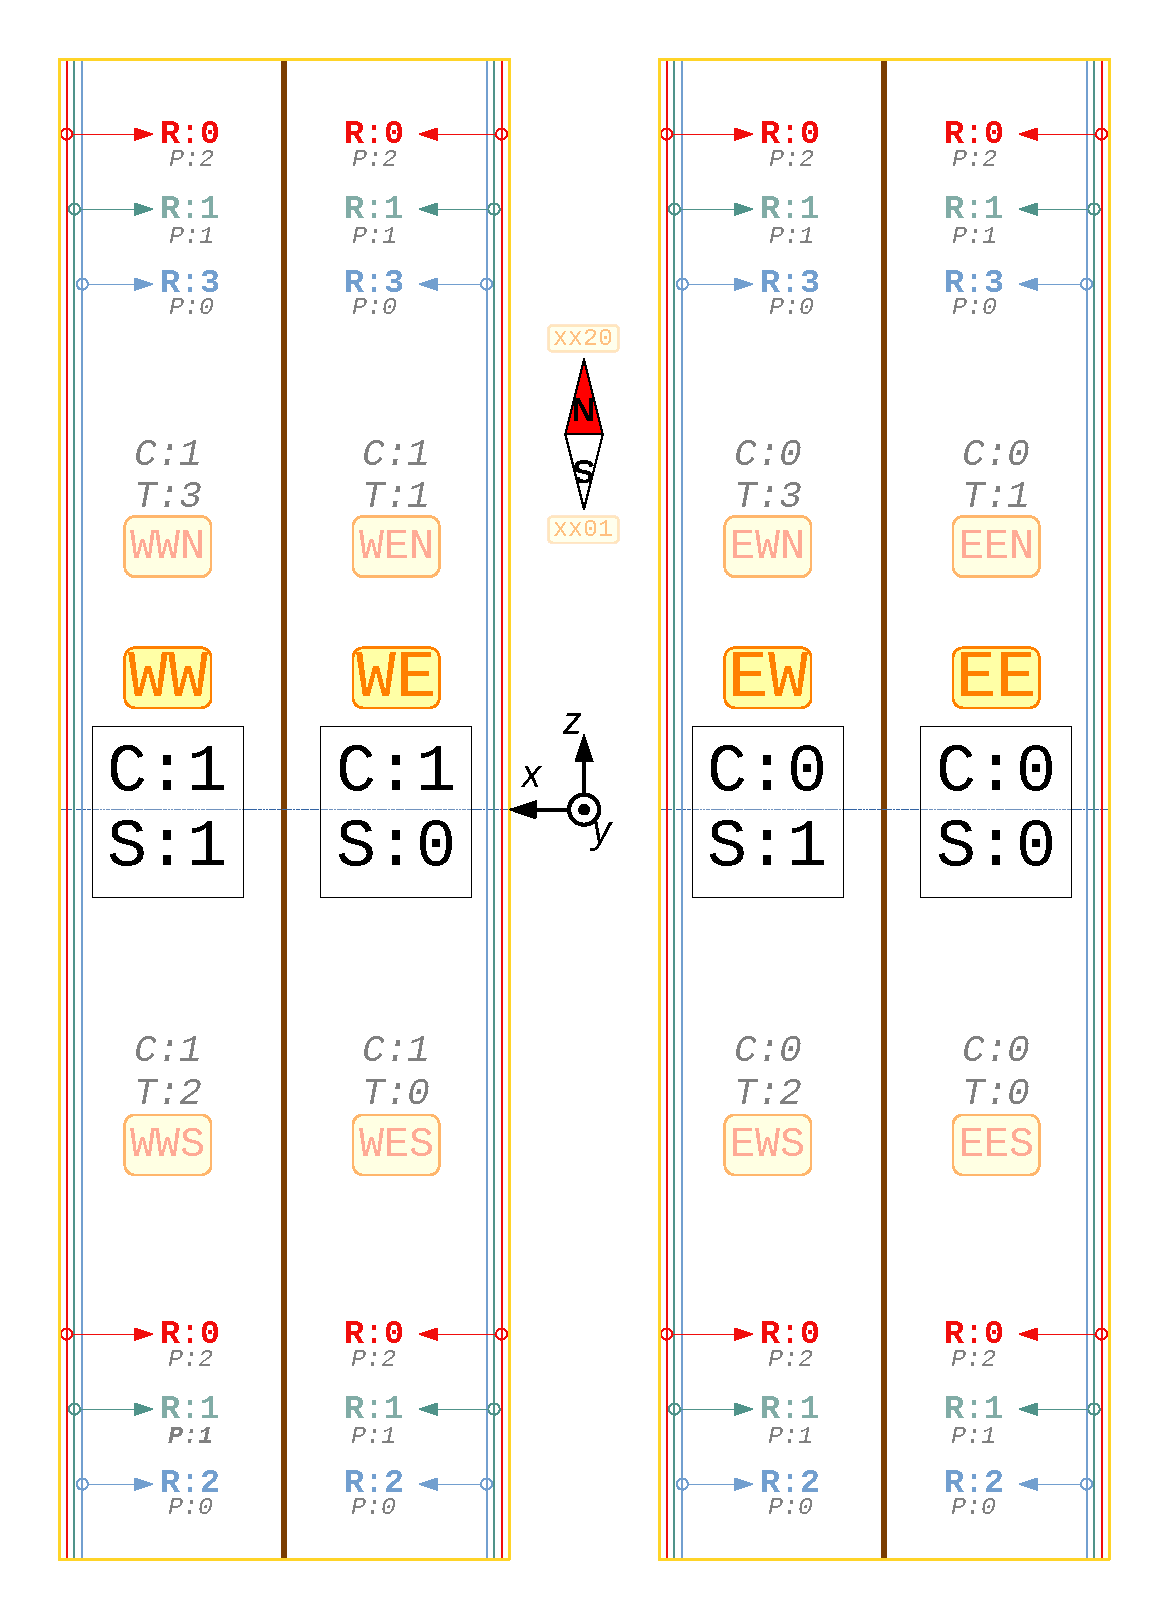
\includegraphics[height=0.90\textheight]{figures/LArSoftLabels}
  \end{center}
  \caption{
    Illustation of detector elements labels and reference frame in LArSoft.
    \label{fig:LArSoftLabels}
  }
\end{figure}

LArSoft coordinate system has the $x$ axis pointing westward,
the $y$ axis pointing upward and the $z$ axis pointing northward.

LArSoft interprets ICARUS detector as being made of two \emph{cryostats},
identified by a number growing with $x$:
\texttt{C:0} for module \Module{E} and \texttt{C:1} for module \Module{W}.
Each cryostat has two \emph{TPC sets}, and each of them has \emph{four}
\emph{readout planes}.
Each of the LArSoft TPC sets (label \texttt{S}) in ICARUS describes an actual TPC and drift
volume, and includes two LArSoft \emph{logical} TPCs (label \texttt{T}).
TPC sets are also numbered with increasing $x$ coordinate, so that
TPC \TPC{EE} is \texttt{C:0 S:0}, TPC \TPC{EW} is \texttt{C:0 S:1},
TPC \TPC{WE} is \texttt{C:1 S:0} and TPC \TPC{WW} is \texttt{C:1 S:1}.
A LArSoft readout plane (label \texttt{R}) is a group of channels on the same type of plane,
completely contained in a single TPC set.
Each can include one or more logical LArSoft wire planes.
Two of the readout planes count 5728 channels each and cover a complete physical wire
plane: \texttt{R:3} covers the collection plane (including planes numbered \texttt{P:2})
and \texttt{R:2} covers the second induction plane (including planes numbered \texttt{P:1}).
The other two readout planes include each half of the first induction plane (numbered \texttt{P:0}):
\texttt{R:0} for the southern half (``Ind-1-S'', \texttt{T:$2n$ P:0})
and \texttt{R:1} for the northern half (``Ind-1-N'', \texttt{T:$2n+1$ P:0}).

Channels are numbered starting with the first TPC set (TPC set \TPC{C:0 S:0}),
and starting with the readout plane closter to the cathode,
that is the one with the first induction plane, with preferential order first
with increasing $z$ coordinate, and then with increasing $y$ coordinate.
The ``wireless'' channels belong to their respective readout plane:
each second induction and collection readout plane starts with 64 wireless channels,
counts then the regular 5600 channels, then ends with another 64 wireless channels,
including overall 5278 channels.
LArSoft wire planes, on the other end, do not include any wireless channel:
wireless channels are associated only to LArSoft readout planes
and not to LArSoft readout planes.

This translates into the following mapping:
\begin{center}
  \small
  \begin{tabular}{|ccr||ccr|}
    \hline
    \hline
    Location            & LArSoft ROP          & channels     & Location            & LArSoft ROP          & channels     \\
    \hline
    \texttt{EE} Ind-1-S & \texttt{C:0 S:0 R:0} &     0-- 1055 & \texttt{WE} Ind-1-S & \texttt{C:1 S:0 R:0} & 27136--28191 \\
    \texttt{EE} Ind-1-N & \texttt{C:0 S:0 R:1} &  1056-- 2111 & \texttt{WE} Ind-1-N & \texttt{C:1 S:0 R:1} & 28192--29247 \\
    \texttt{EE} Ind-2   & \texttt{C:0 S:0 R:2} &  2112-- 7839 & \texttt{WE} Ind-2   & \texttt{C:1 S:0 R:2} & 29248--34975 \\
    \texttt{EE} Coll    & \texttt{C:0 S:0 R:3} &  7840--13567 & \texttt{WE} Coll    & \texttt{C:1 S:0 R:3} & 34976--40703 \\
    \hline
    \texttt{EW} Ind-1-S & \texttt{C:0 S:1 R:0} & 13568--14623 & \texttt{WW} Ind-1-S & \texttt{C:1 S:1 R:0} & 40704--41759 \\
    \texttt{EW} Ind-1-N & \texttt{C:0 S:1 R:1} & 14624--15679 & \texttt{WW} Ind-1-N & \texttt{C:1 S:1 R:1} & 41760--42815 \\
    \texttt{EW} Ind-2   & \texttt{C:0 S:1 R:2} & 15680--21407 & \texttt{WW} Ind-2   & \texttt{C:1 S:1 R:2} & 42816--48543 \\
    \texttt{EW} Coll    & \texttt{C:0 S:1 R:3} & 21408--27135 & \texttt{WW} Coll    & \texttt{C:1 S:1 R:3} & 48544--54271 \\
    \hline
    \hline
  \end{tabular}
\end{center}
In the collection and second induction planes channel numbering within the plane
starts from south (negative $z$).
For the first induction plane, channel numbering starts from the bottom instead
(negative $y$ direction).

LArSoft wire planes are traditionally numbered starting from the plane closest
to the cathode, numbered as \texttt{P:0}.
In this mapping, four readout planes are required grouping six wire planes:
two readout planes contain two wire planes each (second induction and collection planes)
and the other two contain one wire plane each.

